\documentclass[../main.tex]{subfiles}

\begin{document}

Unter einer General Purpose x86 CPU werden Prozessoren verstanden, die den Befehlssatz und die Architektur x86 verwenden. Diese Architektur wird von den beiden großen CPU Herstellern Intel und AMD verwendet und befindet sich somit in nahezu allen PCs und Laptops. 

Heutige CPUs dieser Hersteller verstehen wesentlich mehr Instruktionen als der klassische x86-Befehlssatz. Somit bestehen heute einige Möglichkeiten, den Programmcode für diese Architektur zu optimieren. Eine dieser Optimierungsmöglichkeiten ist die Verwendung von SIMD-Instruktionen (Single Instruction, Multiple Data). Damit können mehrere Rechenoperationen gleichzeitig in speziellen Registern ausgeführt werden.

Zur Entwicklung des Programms wurde Eclipse CDT verwendet und als Compiler gcc, ein weit verbreiteter Compiler mit einer großen Open Source Comunity. 

\section{OpenMP (Open Multi Procesing)}

Aktuelle CPUs, ob im Arbeitsrechner, Laptop, Tablet oder Smartphone, besitzen inzwischen mehrere CPU-Kerne. Um das volle Potenzial der dieser CPUs auszunutzen ist es zwingend notwendig, Programme zu parallelisieren, sodass Programmabschnitte auf mehreren Kernen gleichzeitig ausgeführt werden können.
„Unter der Parallelisierung eines Programms versteht man, dass mehrere Teile einer Aufgabe gleichzeitig nebeneinander ausgeführt werden, um so die Gesamtaufgabe schneller als bei strikt serieller Verarbeitung zu beenden. \cite{articleOpenMP}"

Mit der Programmierschnittstelle OpenMP ist es relativ einfach Programme, mithilfe von Direktiven die in den Programmcode eingefügt werden, parallel ablaufen zu lassen. OpenMP ist hierbei für die Programmiersprachen C, C++ und Fortran verfügbar.

\subsection{Programmiermodell}

Die nebenläufige Abarbeitung von Programmteilen wird bei OpenMP durch das Fork-Join-Prinzip erzielt. Dabei erfolgt an einer bestimmten Stelle im Programmcode ein sogenannter Fork. An dieser Punkt erzeugt der Thread, der den vorherigen Programmcode ausgeführt hat, neue Threads die den danach folgenden Code parallel ausführen. Der Thread, der die anderen Threads erzeugt hat, wird Master-Thread genannt. Am Ende des parallelen Bereichs geschieht ein Join. Bei einem Join werden alle Treads synchronisiert und beendet. Lediglich der Master-Thread bleibt erhalten und führt das weitere Programm seriell aus.

OpenMP erlaubt es auch, einen Fork innerhalb eines parallelen Programmabschnittes zu tätigen. Der außerhalb liegende Join muss dann auf alle innere Joins warten, also bis alle innerhalb erzeugten Threads beendet wurden.

\subsection{OpenMP-Direktiven}

Im folgenden Abschnitt sind alle Programmbeispiele in C- oder C++-Syntax gehalten. Die selben Anweisungen sind auch in Fortran möglich, können sich jedoch in der Erscheinungsweise unterscheiden.

Zuerst muss die Datei \texttt{omp.h} includiert werden. Anschließend kann mit \texttt{\#pragma\ omp\ <Klausel>} eine Compiler-Direktive angegeben werden. Mithilfe dieser Direktive und OpenMP wird der folgende Programmabschnitt parallel ausgeführt. Von Kompilern, die OpenMP nicht unterstützen, wird diese Zeile ignoriert. Somit kann der gleiche Programmcode als paralleles oder als serielles Programm compiliert werden.

\subsubsection{Variablen}

Variablen können entweder privat oder gemeinsam deklariert werden. Eine gemeinsame Variable kann von verschiedenen Threads genutzt werden, während eine private Variable für jeden Thread einen anderen Wert annehmen kann. Gemeinsame Variablen werden mit dem Parameter \texttt{shared(Liste\_der\_Variablen)} deklariert. In der Liste werden alle Variablen hineingeschrieben, die gemeinsam genutzt werden sollen. Die Variablen sind mit dem Wert initialisiert, die sie vor dem Fork hatten. Private Variablen können hingegen mit \texttt{private(Liste\_der\_Variablen)} deklariert werden.  Anders als die Gemeinsamen Variablen sind diese anfangs nicht initialisiert, mit Ausnahme von Objekten die einen Konstruktur besitzen und Indexvariablen von Schleifen.
Soll der Wert, den die Variable vor Beginn der parallelen Ausführung hatte, verwendet werden, muss dafür der Parameter \texttt{firstprivate(Liste\_der\_Variablen)} verwendet werden. Soll der Wert der Variable vor dem Join im weiteren Programmablauf verwendet werden, muss hierfür der Parameter \texttt{lastprivate(Liste\_der\_Variablen)} verwendet werden.

Eine weitere Möglichkeit bei Variablen sind die Reduktionsvariablen. Diese funktionieren wie private Variablen, bis zum Zeitpunkt des Joins. Bei Reduktionsvariablen werden alle Werte der privaten Variablen durch eine Operation zusammengefasst. Bei dieser Operation kann es sich um die Addition, Subtraktion, Multiplikation, XOR, binäre und Logische Und-Verknüpfung oder binäre und Logische Oder-Verknüpfung handeln. Der Parameter für Reduktionsvariablen lautet \texttt{reduction( op:Liste\_der\_Variablen)}.
„Wird eine Variable in keiner der Deklarationen erwähnt, wird sie standardmäßig als gemeinsame Variable deklariert. Eine Ausnahme hiervon bildet die bei der Aufteilung einer Schleife auf mehrere Threads erzeugte Index-Variable der Schleife, die standardmäßig als private Variable deklariert wird. Soll ein explizites Deklarieren jeder im parallelen Bereich verwendeten Variable erzwungen werden, so wird der Direktive zusätzlich der Parameter default(none) hinzugefügt.“ (Uni München)

\subsubsection{Parallelisierung}

Parallele Abschnitte des Programms beginnen immer mit der Direktiven \texttt{\#pragma omp parallel}. Der Folgende Code wird dann parallel ausgeführt, der Code kann beschränkt werden durch die Verwendung von geschwungenen Klammern. Der Auszuführende Code ist hierbei in jedem Thread derselbe. 

Die Nummer des Threads, der den Aktuellen Code ausführt, kann mit \texttt{omp\_get\_thread\_num} ermittelt werden. Die Gesamtanzahl der Threads wird bei Aufruf von \texttt{omp\_get\_num\_threads} zurückgegeben.

Die bei der Implementierung des Neuronalen Netzwerkes am meisten verwendete Direktive von OpenMP ist \texttt{\#pragma omp parallel for [Parameter]}. Diese muss vor eine For-Schleife gesetzt werden. Die For-Schleife wird dann parallel abgearbeitet. Eine Bedingung zur Verwendung dieser Direktiven ist, dass die Anzahl der Durchläufe schon vor Beginn des ersten Durchlaufs berechenbar sein muss. Außerdem darf kein Ergebnis eines vorherigen Schleifendurchlaufs zur Berechnung eines Ergebnis in einem späteren Durchlauf benötigt werden.
Als Parameter kann zum Einen die Schedule-Strategie angegeben werden. 
Für eine statische Strategie, bei der eine Bestimmte Anzahl an Interationen statisch auf die Threads verteilt werden, gibt es den Parameter \texttt{schedule(static, [Blockgröße])}. Die Blockgröße kann Optional angegeben werden. Wird sie nicht angegeben, werden alle Iterationen durch die Anzahl der Threads geteilt und diese Anzahl verwendet.
Bei einer dynamischen Verteilung muss der Parameter \texttt{schedule(dynamic, [Blockgröße])} angegeben werden. Sollten einige Iterationen länger dauern als andere, werden Iterationen auf andere Threads verlegt um zu vermeiden, dass gegen Ende der Abarbeitung ein einziger Thread noch rechnen muss, währenddessen alle anderen Threads schon lange fertig sind.
Die letzte Strategie in OpenMP kann mit der Direktiven \texttt{schedule(guided, [Blockgröße])} verwendet werden. Hierbei werden die Blöcke zur Abarbeitung mit fortschreiten der Zeit immer kleiner. Iterationsblöcke, die schneller fertig werden, bekommen dann einen größeren zweiten Block als Iterationen, die später ihren ersten Block abgearbeitet haben. Die Anzahl der Iterationsblöcke soll dadurch verringert werden.
Bei Beendigung der Schleife wird normalerweise darauf gewartet, bis alle Threads beendet werden können. Soll dies nicht geschehen, kann der Parameter \texttt{nowait} angegeben werden.
Ein weiterer Parameter zur Parallelisierung einer For-Schleife ist \texttt{ordered}. Dabei werden die Iterationen in der Reihenfolge ausgeführt, wie Sie bei paralleler Ausführung ausgeführt würden. Bei diesem Parameter kann noch ein Block mit dem Direktiv \texttt{\#pragma omp ordered} unterhalb der For-Schleife stehen. Dieser wird dann auch in der gleichen Reihenfolge ausgeführt.

Weitere Funktionen zur Parallelisierung mit Hilfe von OpenMP wurden für diese Arbeit nicht verwendet und werden deswegen im Folgenden nur kurz erwähnt.
Für verschiedenen Bereiche, die unabhängig voneinander sind und parallel ausgeführt werden sollen, kann \texttt{\#pragma imp parallel section [Parameter]} verwendet werden.
Für kritische Abschnitte gibt es \texttt{\#pragma omp critical [(name)]} und eine Barriere kann mit \texttt{\#pragma omp barrier} erzeugt werden.

\section{Umsetzung}

Zur Implementierung des Convolutional Neural Networks auf einer x86-Architektur wird die serielle Implementierung als Grundlage verwendet. Diese muss jedoch umgeschrieben werden, um parallel auf mehreren CPU-Kernen verwendet werden zu können. Des weiteren werden folgende Methoden zur Optimierung verwendet:
\begin{itemize}
	\item Reduzierung der Speicherzugriffe
	\item Cache-Hierarchie ausnutzen
	\item AVX zur Multiplikation verwenden
\end{itemize}

\subsection{Optimierung des Convolutional Layers}

Die größten Optimierungsmöglichkeiten ergeben sich im Convolutional Layer. Bei der seriellen Implementierung wird für jede Multiplikation ein neues Array beschrieben, welches dann mit einem Gewichts-Array multipliziert wird. Das Ergebnis dieser Multiplikation wird dann in eine temporäre Variable gespeichert, zu welcher dann ein Bias addiert wird um am Ende den Wert für den Output zu erhalten. Die Vorgehensweise ist in der Grafik unterhalb zu sehen.

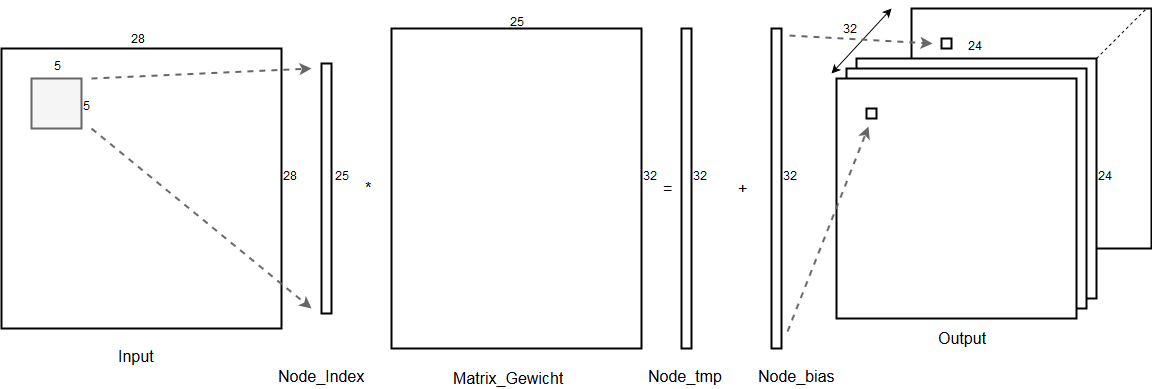
\includegraphics[width=\textwidth]{../images/Benz/Conv_Layer_Seriel.png} %Grafik Ablauf Convolutional Layer Seriell

Aus einem Input wird der Bereich ausgewählt, der mit dem Kern gefaltet werden soll. Die entsprechenden Werte werden in einen neuen Vektor geschrieben. Dieser Vektor wird anschließend mit dem Kern Multipliziert. Das Ergebnis wird in einen temporären Vektor geschrieben und anschließend noch mit dem Bias-Vektor elementweiße multipliziert. Die dabei entstehenden Werte werden an die richtige Stelle der Output-Matrix geschrieben.

Bei dieser Vorgehensweise sind sehr viele neue Allokationen des Hauptspeichers nötig, da viel Speicherplatz kurzfristig benötigt wird. Dies kann sich vermeiden lassen, indem man die Multiplikationen geschickt nacheinander ausführt und das Ergebnis direkt in den Zielspeicherplatz schreibt. 

Es wurde sich für eine Methode entschieden, bei der jedes Element vom Activation-Tensor durchgegangen wird. Hierbei wird zuerst der Output-Tensor auf 0 gesetzt. Je nachdem, wo sich das Element im Activation-Tensor befindet, gibt es verschiedene Elemente der Gewichts-Matritzen, mit denen es multipliziert werden muss. Das erste Element links oben muss nur mit dem Element links oben des Faltungskerns multipliziert werden, währenddessen Elemente in der Mitte des Input-Tensors mit allen Elementen des Faltungskerns multipliziert werden müssen und die Ergebnisse an verschiedenen Stellen im Output geschrieben werden. Die entsprechenden Elemente des Faltungkerns werden mit zwei if-Bedingungen ermittelt. Anschließend werden diese Werte des Faltungskerns mit dem einen Element des Inputs multipliziert und die Ergebnisse an die richtige Stelle des Output-Tensors hinzugefügt.

In unten stehender Formel ist der Vorgang zu erkennen. x\_pos und y\_pos sind die Indizes des Faltungskerns mit dem das Element \(a_{x,y,z}\) multipliziert werden muss. Alle Kombinationen von x\_pos, y\_pos und z\_pos werden durchgegangen. Anschließend wird das nächste Element von \(a\) verwendet.
\begin{equation}
\begin{split}
x\_pos = {min\_x_{a_{x,y,z}}\ ..\ max\_x_{a_{x,y,z}}}\\
y\_pos = {min\_y_{a_{x,y,z}}\ ..\ max\_y_{a_{x,y,z}}}\\
z\_pos = {z\ ..\ length(w_{z})\ [SW:\ length(a_{z})]}\\
o_{x-x\_pos,y-y\_pos,z\_pos/z} += a_{x,y,z}*w_{x\_pos,y\_pos,z\_pos}
\end{split}
\end{equation}

Durch diese Methode kann der Output-Tensor und die Gewichte im Cache liegen, die Speicherzugriffe erfolgen somit sehr schnell. Da kein neuer Speicher allokiert wird, muss nicht darauf gewartet werden bis der vergleichsweise sehr langsame Arbeitsspeicher den Speicherplatz freigibt und die Daten in den Cache geladen werden können. 

\subsubsection{Alternative Implementierung des Convolutional Layers}

Der Convolutional Layer kann auf mehrere Arten Implementiert werden. Immer müssen mehrere For-Schleifen ineinander die Faltung mit dem Faltungskern ausführen, dazu werden die einzelnen Zählvariablen als Index des Input und des Outputs verwendet. Es kann jedoch entschieden werden, welche Variable für welchen Indes verwendet wird.

Die wohl einfachste Art der Implementierung ist die, dass die äußeren For-Schleifen den Index des Outputs bestimmen und die inneren den Index des Inputs und des Faltungskerns. Bei dieser Art kann der Index des Outputs als Anfangsindex des Inputs verwendet werden. Die inneren Schleifen erzeugen einen Offset zwischen 0 und der Breite/Länge des Faltungskerns. Dieser Offset wird auf die Variable des Outputs addiert und erzeugt somit die Positionen des Inputs, die für den Output verwendet werden.

OpenMP
-> kritische Abschnitte
-> Barriere
-> ...

Alternative Methoden zu Forward
-> Gewichte durchgehen
-> Quellcode
-> Output-Layer durchgehen

Aufbau Programm
-> Layer Vererben, gleiche Funktionen forward(), backward()
-> Noch im Programmcode ändern

AVX
-> set\_ps --> andersherum in Register



\subsection{Verwendung von AVX}

Eine weitere Optimierung ergibt sich durch die Verwendung von AVX (Advanced Vector Extensions).  Neue CPUs von Intel und AMD besitzen spezielle AVX-Register. Auf diese Register können SIMD (Single Instruction Multiple Data) Operationen angewandt werden. AVX ist der Nachfolger von SSE (Streaming SIMD Extension). Einer dieser SIMD Operationen ist die Multiplikation von float Zahlen.
Je nach Generation des Prozessors sind die AVX-Register 256 oder 512 Bit groß. Bei älteren Prozessoren mit SSE haben die Register eine Größe von 128 Bit. Somit lassen sich bei neueren Generationen bis zu 16 Floats in einem Register unterbringen. Für die Multiplikation werden 2 Register benötigt, die mit den zu multiplizierenden Floats initialisiert sind. Durch Aufrufen des Befehls zur Multiplikation werden nun das n-te Float in Register a mit dem n-ten Float in Register b multipliziert und in ein Zielregister geschrieben.

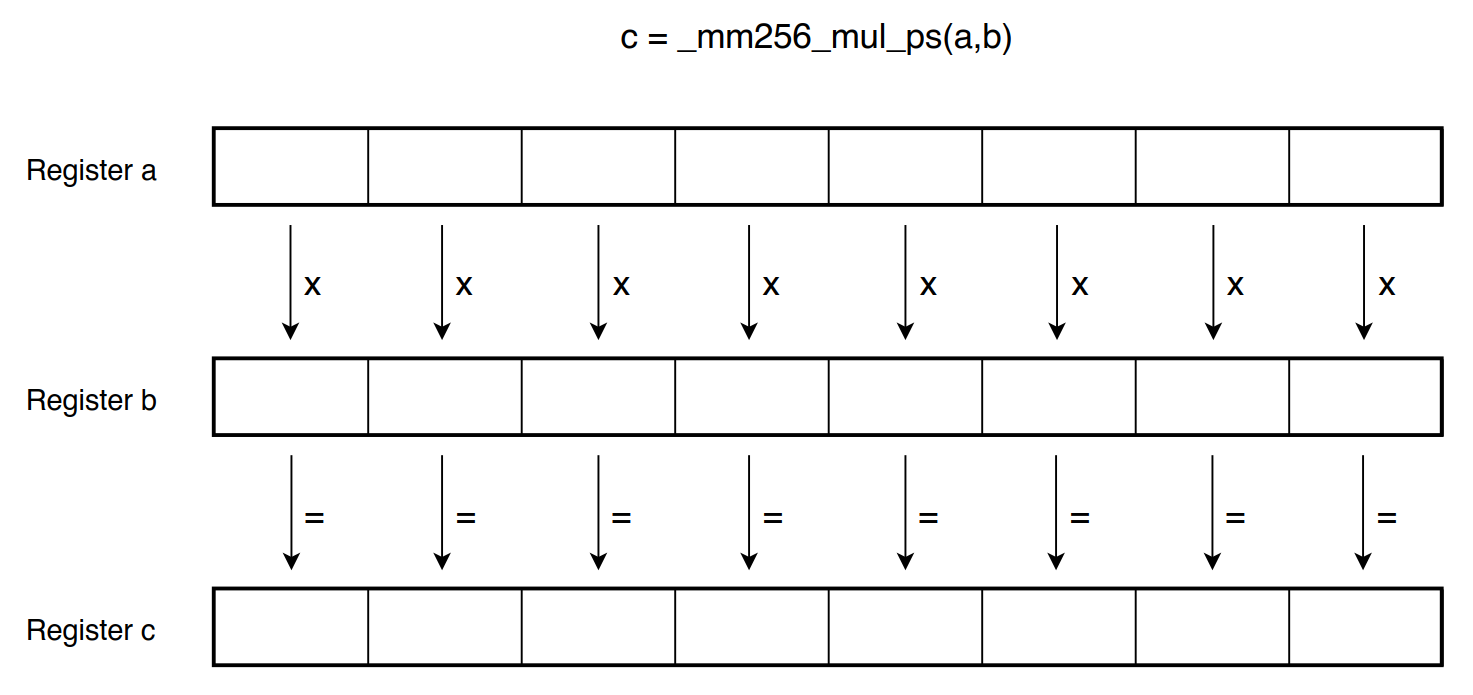
\includegraphics[width=\textwidth]{../images/Benz/avx.png}

In der Grafik werden 8 Multiplikationen von Floats mit der Instruktion \texttt{\_mm256\_mul\_ps()} gleichzeitig ausgeführt. Die \texttt{256} gibt hierbei an, wie groß die Register sind. In diesem Fall sind die Register 256 Bit groß. Anschließend wird die Rechenart angegeben, hier eine Multiplikation (\texttt{mul}). Das \texttt{p} steht für "packed". Hierbei werden im Register mehrere Floats erwartet. Alternativ kann ein \texttt{s} für "single slot" angegeben werden, dann wird lediglich die hinterste Position des Registers für die Multiplikation verwendet. An letzter Stelle steht ein \texttt{s}. Dieses steht für "single precision", also für den Datentyp Float. Bei einem \texttt{d}an dieser Stelle werden Doubles angenommen, die Anzahl der gleichzeitigen Multiplikationen halbiert sich dadurch, dafür wächst der Wertebereich der Zahlen.

Eine Übersicht aller SIMD-Instruktionen von Prozessoren mit aktueller x86-Architektur und findet sich unter \url{https://software.intel.com/sites/landingpage/IntrinsicsGuide}. 

Durch die Verwendung von AVX lässt sich somit die Zeit zum Multiplizieren von mehreren Zahlen, im Vergleich zur standardmäßigen Multiplikation, bis zu 16 mal verkürzen. Der gcc-Compiler versucht auf Optimierungsstufe 3 for-Schleifen automatisch zu vektorisieren. Deswegen ist es nicht unbedingt vonnöten, die AVX-Register mühsam selbst zu verwenden. Durch das Compiler-Flag \texttt{-ftree-vectorizer-verbose=2} wird bei jeder Schleife ausgegeben, ob gcc den Code vektorisieren konnte und somit den Code mit SIMD-Instruktionen übersetzt hat.

Die Instruktionen können jedoch auch explizit aufgerufen werden, sodass nicht der Compiler die Entscheidung übernimmt, wo und wie optimiert werden soll, sondern dies der Programmierer selbst Entscheiden kann. 


\end{document}